\setcounter{figure}{0}
\renewcommand{\figurename}{S-Fig.}
\setcounter{table}{0}
\renewcommand{\tablename}{S-Tab.}
\def\V{\mathds{V}}
\def\Appendix{Appendix}
%###################################

\newif\iftikzX
\tikzXtrue
\tikzXfalse
%--------------
\def\jobnameX{zero}
%--------------
\newif\ifFIGS
\FIGSfalse 
\FIGStrue
%--------------
\newif\ifdraftQ
\draftQtrue
%\draftQfalse
%--------------
%###################################
\def\TITLE{\LARGE \enet: Fast Scalable Pandemic Risk Estimation of  \infl Strains Collected In Non-human Hosts}
%\def\TITLE{\LARGE A Biologically Meaningful Sequence Metric\\For Analyzing Evolutionary Changes\\In Novel Pathogens}
%\def\TITLE{Learning  Mutational Patterns At Scale For\\Analysis Of Sequence Divergence\\In Novel Pathogens}
%\def\TITLE{Learning Mutational Patterns at Scale to Analyze Sequence Divergence in Novel Pathogens}

\def\authore{Kevin Wu}
\def\authora{ Jin Li}
\def\authorb{Timmy Li}
\def\authorc{Aaron Esser-Kahn}
\def\authord{Ishanu Chattopadhyay}

\def\addressa{Department of Medicine, University of Chicago, IL, USA}
\def\addressb{Committee on Genetics, Genomics \& Systems BioloScalegy, University of Chicago, IL, USA}
\def\addressc{Committee on Quantitative Methods in Social, Behavioral, and Health Sciences, University of Chicago, IL, USA}
\def\addressd{Pritzker School of Molecular Engineering, University of Chicago, Chicago, IL, USA}
\def\addresse{Committee on Immunology, University of Chicago, Chicago, IL, USA}
\newif\ifdraftQ
\draftQtrue
\draftQfalse


%###################################

\title{\TITLE}
\author{\sffamily  \fontsize{10}{12}\selectfont   \authore$^{1}$,\authora$^{1}$, \authorb$^{1}$,  \authorc$^{2,3}$, and \authord$^{1,4,5\bigstar}$\\                                                                
\vspace{10pt}                                                                   

\sffamily  \fontsize{10}{12}\selectfont                                         
$^{1}$\addressa\\   
$^{2}$\addressd\\
$^{3}$\addresse\\
$^{4}$\addressb\\
$^{5}$\addressc                                                                 
\vskip 1em                                                                      
$^\bigstar$To whom correspondence should be addressed: e-mail: \texttt{ishanu@uchicago.edu}.}


\def\hcov{SARS-CoV-2\xspace}
\def\RATG13{RaTG13\xspace}
\def\Appendix{Appendix}
\def\qnet{Qnet\xspace}
\def\enet{Emergenet\xspace}
\def\erisk{risk\xspace}
\def\qdist{E-distance\xspace}
\def\cov{COVID-19\xspace}
\def\infl{Influenza A\xspace}
%\def\infl{IAV\xspace}


\def\E{\mathcal{E}}
\def\dst{x_\star^{t+\delta}}
\def\dsta{x^{t+\delta}}

%\setcounter{table}{0}
%\renewcommand{\tablename}{SI Tab.}

%#############################################
%#############################################
\begin{table}[!ht]
\mnp{\textwidth}{  \centering
 \captionN{Number of Influenza sequences collected from public databases}\label{tabseq}
\sffamily\fontsize{8}{8}\selectfont
\begin{tabular}{L{.7in}|L{1.55in}|L{.95in}}\hline
Database & Strain & No. of Sequences \\\hline
NCBI& Influenza  H1N1  HA &17,894\\\hline
NCBI& Influenza  H1N1  NA &16,637\\\hline
NCBI& Influenza  H3N2  HA &18,265\\\hline
NCBI& Influenza  H3N2  NA &14,699\\\hline
GISAID& Influenza  H1N1  HA &1,528\\\hline
GISAID& Influenza  H1N1  NA &1,490\\\hline
GISAID& Influenza  H3N2  HA &13,975\\\hline
GISAID& Influenza  H3N2  NA &13,811\\\hline
Total & &98,299\\\hline
\end{tabular}
}
\end{table}
% #############################################


%#############################################
%#############################################
\begin{table*}[!ht]
\def\ACOL{teal!30}
\def\BCOL{Red1!30}
\def\CCOL{gray!30}
\captionN{Examples: \enet induced distance varying for fixed sequence pair when background population changes (rows 1 -5), sequences with small edit distance and large \qdist, and the converse (rows 6-9)}\label{tabex}
\begin{tabular}{L{.1in}|L{.45in}|L{1.85in}|L{2in}|L{.5in}|L{.325in}|L{.325in}}\hline
& Edit dist. & Sequence A & Sequence B & \enet E-dist. & Year A$^\star$ & Year B$^\star$\\\hline
\rowcolor{\ACOL}1&18 & A/Singapore/23J/2007 & A/Tennessee/UR06-0294/2007 & 0.0111 & 2007 & 2007\\\hline
\rowcolor{\ACOL}2&18 & A/Singapore/23J/2007 & A/Tennessee/UR06-0294/2007 & 0.0094 & 2008 & 2008\\\hline
\rowcolor{\ACOL}3&18 & A/Singapore/23J/2007 & A/Tennessee/UR06-0294/2007 & 0.0027 & 2009 & 2009\\\hline
\rowcolor{\ACOL}4&18 & A/Singapore/23J/2007 & A/Tennessee/UR06-0294/2007 & 0.0025 & 2010 & 2010\\\hline
\rowcolor{\ACOL}5&18 & A/Singapore/23J/2007 & A/Tennessee/UR06-0294/2007 & 0.6163 & 2007 & 2010\\\hline
\rowcolor{\BCOL}6&11 & A/Naypyitaw/M783/2008 & A/Singapore/201/2008 &      0.8852 & 2008 & 2008\\\hline
\rowcolor{\BCOL}7&15 & A/Cambodia/W0908339/2012 & A/Singapore/DMS1233/2012&0.2737 & 2012 & 2012\\\hline
\rowcolor{\CCOL}8&126 & A/South Dakota/03/2008 & A/Singapore/10/2008 &     0.3034 & 2008 & 2008\\\hline
\rowcolor{\CCOL}9&141 & A/Jodhpur/3248/2012 & A/Cambodia/W0908339/2012 &   0.2405 & 2012 & 2012\\\hline
\end{tabular}
\flushleft
$^\star$Year A and year B correspond to the assumed collection years for sequences A and B respectively for the purpose of this example. Sequence A in row 1 is collected in 2007, but is assumed to be from different years in rows 2-4 to demonstrate the change in \qdist from sequence B, arising only from a change in the background population.
\end{table*}
%#############################################
%#############################################

%#############################################
%#############################################
\begin{table}[!ht]
 \mnp{\textwidth}{ \centering
 \captionN{Correlation between \qdist and edit distance between sequence pairs}\label{tabcor}
\sffamily\fontsize{8}{8}\selectfont
\begin{tabular}{L{1.35in}|L{.65in}}\hline
Phenotypes & Correlation \\\hline
 Influenza H1N1 HA  &0.76\\\hline
 Influenza H1N1 NA &0.74\\\hline
 Influenza H3N2 HA &0.85\\\hline
 Influenza H3N2 NA &0.79\\\hline
% \hcov &0.52\\\hline
\end{tabular}
}
\end{table}
% #############################################



%#############################################
\ifFIGS
\begin{figure*}[!ht]
  \centering    
  \tikzexternalenable  
  \tikzsetnextfilename{blastvalid}
  %\tikzXtrue
  \iftikzX 
  \def\QCLR{Cyan3}
\def\QCLRB{Cyan3}
\def\RCLR{Tomato}
\def\TEXTCOL{black}
\begin{tikzpicture}[font=\sffamily\fontsize{8}{9}\selectfont]
\clip (-1.5in,2.875in) rectangle (5.75in,-1.75in);
% all text in the axes and labels
\pgfmathdeclarefunction{gauss}{2}{%
  \pgfmathparse{1/(#2*sqrt(2*pi))*exp(-((x-#1)^2)/(2*#2^2))}%
}
  \tikzset{slabel/.style={font=\sffamily\fontsize{11}{5}\selectfont,text=gray}}
  \tikzset{ldr/.style={very thin,Purple3,opacity=.9}}
  \def\LWDT{3pt}
  \def\XST{2.75in}
  \def\INSP{7pt}
  \node[] (A) {
\SetCoordinates[xAngle=-10,yAngle=25]
% ,yLength=1.2,xLength=.8]
\begin{tikzpicture}[scale=.6,multilayer=3d,font=\fontsize{18}{8}\selectfont]
 \def\COLA{Bisque4!80}
\def\COLB{Bisque4!80}
\def\COLC{Bisque4!80}
\def\COLD{Bisque4!80}
 \def\COLA{SlateGray!60}
\def\COLB{SlateGray!60}
\def\COLC{SlateGray!50}
\def\COLD{SlateGray!40}

%\def\TEXTCOL{black}
\def\PWDT{6}
\def\PHGT{7}
 \SetLayerDistance{3.25}
\Plane[x=-.50,y=-.5,width=\PWDT,height=\PHGT,image=Figures/8filename, color=\COLA, ImageAndFill,layer=1,NoBorder]
\Plane[x=-.5,y=-.5,width=\PWDT,height=\PHGT,style={},NoBorder,layer=2,color=\COLB,image=Figures/9filename,ImageAndFill]
\Plane[x=-.5,y=-.5,width=\PWDT,height=\PHGT,NoBorder,layer=3,color=\COLC,image=Figures/10filename,ImageAndFill]
\Plane[x=-.5,y=-.5,width=\PWDT,height=\PHGT,NoBorder,layer=4,color=\COLD,image=Figures/11filename,ImageAndFill]



\begin{Layer}[layer=1]
  \node[,text=black,inner sep=\INSP] (N1) at (3.5,4.25) {};
 \end{Layer}
\begin{Layer}[layer=2]
  \node[,text=black,inner sep=\INSP] (N2) at (1.5,4.5) {};
\end{Layer}
\begin{Layer}[layer=3]
  \node[,text=black,inner sep=\INSP] (N3) at (2.25,4.75) {};
\end{Layer}
\begin{Layer}[layer=4]
  \node[,text=black,inner sep=\INSP] (N4) at (.6,.25) {};
\end{Layer}
\node[slabel,inner sep=6pt] (S0)  at ([yshift=-1.25in,xshift=-.75in]N1.south) {A/swine/Iowa/A02271327/2018};
\node[slabel,inner sep=6pt] (S1)  at ([yshift=-.55in,xshift=1in]N1.south) {A/swine/Iowa/A02157799/2018};
\node[slabel,inner sep=6pt] (S2)  at ([yshift=-.8in,xshift=1.7in]N2.south) {A/swine/Iowa/A02268335/2018};
\node[slabel,inner sep=6pt] (S3)  at ([yshift=-.75in,xshift=1.35in]N3.south) {A/swine/Iowa/A02270007/2018};
\node[slabel,inner sep=6pt] (S4)  at ([yshift=.65in,xshift=1.35in]N4.south) {A/swine/Iowa/A02429801/2019};

\draw [opacity=.3,dashed,very thick] (S0.north) -- (N1) -- (N2) -- (N3) -- (N4);
\draw [ldr,] (S1) -- (N1);
\draw [ldr,] (S2) -- (N2);
\draw [ldr,] (S3) -- (N3);
\draw [ldr,] (S4) -- (N4);

\end{tikzpicture}};
\node[circle,draw=IndianRed3,fill=IndianRed3,path fading=fade out,ultra thick,inner sep=6pt,,font=\rm\sffamily\fontsize{6}{8}\selectfont,label={[font=\rm\sffamily\fontsize{8}{8}\selectfont]0:Random Mutations}] (L) at ([xshift=0.5in,yshift=.42in]A.north west) { };
\node[anchor=west,circle,font=\rm\sffamily\fontsize{8}{8}\selectfont,,draw=Cyan1,fill=Cyan1,ultra thick,inner sep=5pt,label={[font=\rm\sffamily\fontsize{8}{8}\selectfont]0:E-Sampled Mutations}] (L1) at ([xshift=1.1in]L.east) { };
\node[anchor=north west,circle,font=\rm\sffamily\fontsize{8}{8}\selectfont,text width=.15in,,label={[font=\rm\sffamily\fontsize{8}{8}\selectfont]0:Possible Evolutionary Trajectory}] (L1111) at ([xshift=0in,yshift=-.05in]L.south west) { };
\draw [dashed, ultra thick,lightgray] (L1111.west) -- (L1111.east);
\node[anchor=center,circle,draw=none,path fading=fade out,,fill=Purple1,ultra thick,inner sep=6pt,opacity=.8] (L11) at (L1) { };
\draw[-{Latex[length=4mm]},ultra thick,opacity=.5,Bisque4!70,text opacity=1] ([xshift=.6in,yshift=.6in]A.south west) -- ([xshift=.6in]$(A.south west)!.75!(A.north west)$) node [midway,sloped,above] {Iterations};
    \def\WDT{1in} % width 
    \def\HGT{1.125in} % height

\node[anchor=north west] (A1) at ([yshift=.6in,xshift=0.1in]A.north east) {
  \begin{tikzpicture}[anchor=center,%font=\bf\sffamily\fontsize{8}{8}\selectfont
    ]
    \def\DATAQNET{Figures/plotdata/qnet_mean.csv}
    \def\DATARANDOM{Figures/plotdata/random_mean.csv}%define datafile

    \begin{axis}[\TEXTCOL, legend columns=2,legend style={text=black,anchor=west,at={(-.5,1.2)},
        inner sep=1pt,draw=none,fill=black!5,fill opacity=.75,align=right,
        text opacity=1,/tikz/column 2/.style={
                column sep=5pt,
            },},
      name=X0,
      % at=(F.south west),
      %xshift=0in,
      %yshift=-0.1in,
      anchor=center,
      width=\WDT,
      height=\HGT,
      scale only axis=true,
      enlargelimits=false,
      enlarge y limits=0.1,
      enlarge x limits=0.04,
      axis on top=false,
      axis line style={black!2, very thick},
      grid,
      xmax=4, 
      ymin=1500,
      grid style={opacity=.95,dashed,very thick,black!10},
      major tick length=0pt,
      ytick style={draw=none},
      scaled y ticks = false,
      y tick label style={/pgf/number format/fixed,
        /pgf/number format/1000 sep = \empty % \thinspace optional
      },
      x tick label style={/pgf/number format/fixed,
        /pgf/number format/1000 sep = \empty % Optional
      },
      ylabel={p-blast score},xlabel={iteration step},ylabel style={yshift=-.1in},xlabel style={yshift=.05in},]
      
      \addplot [smooth,ultra thick,
      draw=\QCLRB,mark=*,mark options={scale=2.5,draw=white, fill=\QCLR}]
      table [col sep=comma,x=step,y=mean] {\DATAQNET};
      \addlegendentry{Q-sampled}
      
      \addplot [smooth,ultra thick,
      draw=\RCLR,mark=*,mark options={scale=2.5,draw=white, fill=\RCLR}]
      table [col sep=comma,x=step,y=mean] {\DATARANDOM};
      \addlegendentry{Random}
     
    \end{axis}
  \end{tikzpicture}};


\node[anchor=south west] (A2) at ($(A.south west)!(A1.west)!(A.south east)$) {
\begin{tikzpicture}[anchor=center]
\def\QCLR{Cyan3}
\def\QCLRB{Cyan3}
\def\RCLR{Tomato}
\def\TEXTCOL{black}
    \def\WDT{1in} % width 
    \def\HGT{1.25in} % height
\def\DATAVAR{Figures/plotdata/variances.csv}
\begin{axis}[\TEXTCOL, legend columns=2,legend style={text=black,anchor=west,at={(-.5,1.2)},
        inner sep=1pt,draw=none,fill=black!5,fill opacity=.75,align=right,
        text opacity=1,/tikz/column 2/.style={
                column sep=5pt,
            },},name=X1,
      % at=(F.south west),
      %xshift=0in,
      %yshift=-0.1in,
      xmax=4,
      anchor=center,
      width=\WDT,
      height=\HGT,
      scale only axis=true,
      enlargelimits=true,
      enlarge y limits=0.1,
      enlarge x limits=0.04,
      axis on top=false,
      axis line style={black!2, very thick},
      grid,
      grid style={opacity=.95,dashed,ultra thick,black!10},
      major tick length=0pt,
      ytick style={draw=none},
      scaled y ticks = true,
      %y tick label style={/pgf/number format/fixed,
      %  /pgf/number format/1000 sep = \empty % \thinspace optional
      %},
      %x tick label style={/pgf/number format/fixed,
      %  /pgf/number format/1000 sep = \empty % Optional
      %},
      ylabel={variance},xlabel={iteration step},ylabel style={yshift=-.1in},xlabel style={yshift=.05in}]
      \addplot [smooth,ultra thick,
      draw=\QCLRB,mark=*,mark options={scale=2.5,draw=white, fill=\QCLR}]
      table [col sep=comma,x=step,y=qnetvariance] {\DATAVAR};
      \addlegendentry{Q-sampled}
      \addplot [smooth,ultra thick,
      draw=\RCLR,mark=*,mark options={scale=2.5,draw=white, fill=\RCLR}]
      table [col sep=comma,x=step,y=randomvariance] {\DATAVAR};
      \addlegendentry{Random}
\end{axis}
\end{tikzpicture}
};


\node[anchor=north west] (A3) at  ([xshift=.1in]A1.north east) {
\begin{tikzpicture}[anchor=center]
\def\QCLR{teal}
\def\QCLRB{teal}
\def\LCLR{black}
\def\TEXTCOL{black}
    \def\WDT{1.25in} % width 
    \def\HGT{1.125in} % height
\def\DATADIS{Figures/plotdata/dist_between_centers.csv}
\begin{axis}[\TEXTCOL, legend columns=2,legend style={text=black,anchor=west,at={(-.275,1.2),},
        inner sep=1pt,draw=none,fill=black!5,fill opacity=.75,align=right,
        text opacity=1,/tikz/column 2/.style={
                column sep=5pt,
            },},name=X1,
      % at=(F.south west),
      %xshift=0in,
      %yshift=-0.1in,
      xmax=4,
      anchor=center,
      width=\WDT,
      height=\HGT,
      scale only axis=true,
      enlargelimits=true,
      enlarge y limits=0.08,
      enlarge x limits=0.04,
      axis on top=false,
      axis line style={black!2, very thick},
      grid,
      grid style={opacity=.950,dashed,ultra thick,black!10},
      major tick length=0pt,
      ytick style={draw=none},
      scaled y ticks = true,
      %y tick label style={/pgf/number format/fixed,
      %  /pgf/number format/1000 sep = \empty % \thinspace optional
      %},
      %x tick label style={/pgf/number format/fixed,
      %  /pgf/number format/1000 sep = \empty % Optional
      %},
      ylabel={distance [\% increase]},xlabel={iteration step},ylabel style={yshift=-.1in},xlabel style={yshift=.05in}]
      \addplot [smooth,ultra thick,
      draw=\QCLRB,mark=*,mark options={scale=2.5,draw=white, fill=\QCLR}]
      table [col sep=comma,x=step,y expr={100*(\thisrow{qdistance}*625 -1) }] {\DATADIS};
      \addlegendentry{\qdist}
      \addplot [smooth,ultra thick,
      draw=\LCLR,mark=*,mark options={scale=2.5,draw=white, fill=\LCLR}]
      table [col sep=comma,x=step,y expr={100*(\thisrow{ldistance}*0.015 - 1)}] {\DATADIS};
      \addlegendentry{Edit metric}
\end{axis}
\end{tikzpicture}};

\node[anchor=south west] (A4) at ($(A.south west)!(A3.west)!(A.south east)$) {\begin{tikzpicture}[anchor=center]
\def\DATA{Figures/plotdata/year.csv}
    \def\WDT{1in} % width 
    \def\HGT{1.35in} % height
\begin{axis}[, legend columns=2,legend style={text=black,anchor=west,at={(-.2,1.125)},
        inner sep=1pt,draw=none,fill=black!5,fill opacity=.75,align=right,
        text opacity=1,/tikz/column 2/.style={
                column sep=5pt,
            },},
      name=X3,
      xshift=0in,
      yshift=-0.1in,
      anchor=center,
      width=\WDT,
      height=\HGT,
      scale only axis=true,
      enlargelimits=false,
      enlarge y limits=0.150,
      axis on top=false,
      axis line style={black!2, ultra thick},
      grid,
      %xmin=2001,
      %ymax=2019.5,
      grid style={opacity=.95,dashed,ultra thick,black!10},
      % xticklabel style={xshift=0.05in,yshift=-.05in},
      xlabel style={yshift=.05in,text=\TEXTCOL},
      ylabel style={align=center,,text=\TEXTCOL,anchor=center,
        yshift=-.05in},
      % tickpos=left,
      ytick align=outside,
      xtick align=outside,
      major tick length=0pt,
      scaled y ticks = false,
      y tick label style={/pgf/number format/fixed,
        /pgf/number format/1000 sep = \thinspace % Optional 
      },
      x tick label style={/pgf/number format/fixed,
        /pgf/number format/1000 sep = \thinspace % Optional  
      },
      ylabel={year}, xlabel={probability},xbar,bar width=6pt]
      \addplot [fill=\QCLR,draw=none]table [col sep=comma,y=year,x=qnet] {\DATA};
      \addlegendentry{Q-sampled}

      \addplot [fill=\RCLR,draw=none]table [col sep=comma,y=year,x=random] {\DATA};
      \addlegendentry{Random}


\end{axis}

\end{tikzpicture}
};

% \node [anchor=north west] (A5) at ([xshift=.1in,yshift=-.3in]A.south west) {
% \def\COLX{lightgray}
%   \begin{tikzpicture}[anchor=center,square/.style={regular polygon,regular polygon sides=4}]
%   \def\HGT{.3in}
%   \def\WDT{1in}
%   \def\DATAFIRST{Figures/plotdata/first.csv}
% \def\DATASECOND{Figures/plotdata/second.csv}
% \def\DATATHIRD{Figures/plotdata/third.csv}
%   \tikzset{barst/.style={thick,fill=\COLX,ybar,bar width=6pt}}

%   \pgfplotsset{axm/.style={axis line style={draw=none},
%     xlabel={},
%     xticklabel style={rotate=0,xshift=-0.25cm},
%     ylabel={},
%     ylabel style={},
%     ymax=1,
%     yticklabel style={rotate=0,xshift = -0.25cm},
%     height = \HGT,
%     width = \WDT,      scale only axis=true,
%     enlargelimits=false,
%     enlarge y limits=0.02,
%       enlarge x limits=0.150,
%       axis on top=false,
%       axis line style={black!2, ultra thick},
%       %grid,
%        grid style={opacity=.95,dashed,ultra thick,black!10},
%       % xticklabel style={xshift=0.05in,yshift=-.05in},
%       xlabel style={yshift=-0.05in,text=\TEXTCOL},
%       ylabel style={align=center,,text=\TEXTCOL,anchor=center,
%         yshift=-.05in},
%       % tickpos=left,
%       ytick align=outside,
%       xtick align=outside,
%       major tick length=0pt,
%       scaled y ticks = false,
%       y tick label style={/pgf/number format/fixed,
%         /pgf/number format/1000 sep = \thinspace % Optional 
%       },
%       x tick label style={anchor=north, xshift=7pt,yshift=-.02in },
%       ytick={0,0.5,1}}}

%     \node[font=\bf\Large] at (-1,-.15) {$\ldots$};
%     \node at (0,0) [square,draw,label=above:P161] (v161) {X};
%     \node at (1,0) [square,draw,label=above:P162,fill=IndianRed1] (v162) {E};
%     \node at (2,0) [square,draw,label=above:P163] (v163) {N};
%     \node[font=\bf\Large] at (3,-.15) {$\ldots$};
%     \node at (4,0) [square,draw,label=above:P220] (v220) {R};
%     \node at (5,0) [square,draw,label=above:P221,fill=IndianRed1] (v221) {S};
%     \node at (6,0) [square,draw,label=above:P222] (v222) {Y};
%     \node[font=\bf\Large] at (7,-.15) {$\ldots$};
%     \node at (8,0) [square,draw,label=above:P286] (v286) {T};
%     \node at (9,0) [square,draw,label=above:P287] (v287) {S};
%     \node at (10,0) [square,draw,label=above:P288] (v288) {V};
%     \node[font=\bf\Large] at (11,-.15) {$\ldots$};

%     \draw [-{Latex},thick] (v162) -- ++(0,-.275in) node[below,text=Red1] (e162) {K};
%     \draw [-{Latex},thick] (v221) -- ++(0,-.275in) node[below,text=Red1] (e221) {R};
%     \draw [-{Latex},thick,opacity=0] (v287) -- ++(0,-.275in) node[below] (e287) {S};
    
%     \begin{axis}[at={(e162.south)},anchor=north,
%       yshift=0.15in,
%     symbolic x coords={K,R,E,L,N},
%     xtick = {K,R,E,L,N},
%     axm
%      ]
%     \addplot [barst,fill=IndianRed1]table [col sep=comma,x=classes,y=step3] {\DATAFIRST};
%     \end{axis}
    
%     \begin{axis}[at={(e221.south)},anchor=north,
%       yshift=0.15in,
%     symbolic x coords={Y,X,K,R,S},
%     xtick = {Y,X,K,R,S},axm
%     ]
%     \addplot [barst,fill=IndianRed1]table [col sep=comma,x=classes,y=step3] {\DATASECOND};
%     \end{axis}
    
%     \begin{axis}[at={(e287.south)},anchor=north,
%       yshift=0.15in,
%     symbolic x coords={H,L,Q,P,S,V},
%     xtick = {H,L,Q,P,S,V},
%     axm,      enlarge x limits=0.1250,]
%     \addplot [barst]table [col sep=comma,x=classes,y=step3] {\DATATHIRD};
%     \end{axis}
% \end{tikzpicture}
% };



% \node [anchor=north west] (A6) at ([xshift=0in,yshift=-.1in]A5.south west) {
% \def\COLX{lightgray}
%   \begin{tikzpicture}[anchor=center,square/.style={regular polygon,regular polygon sides=4}]
%   \def\HGT{.3in}
%   \def\WDT{1in}
%   \def\DATAFIRST{Figures/plotdata/first.csv}
% \def\DATASECOND{Figures/plotdata/second.csv}
% \def\DATATHIRD{Figures/plotdata/third.csv}
%   \tikzset{barst/.style={thick,fill=\COLX,ybar,bar width=6pt}}

%   \pgfplotsset{axm/.style={axis line style={draw=none},
%     xlabel={},
%     xticklabel style={rotate=0,xshift=-0.25cm},
%     ylabel={},
%     ylabel style={},
%     ymax=1,
%     yticklabel style={rotate=0,xshift = -0.25cm},
%     height = \HGT,
%     width = \WDT,      scale only axis=true,
%     enlargelimits=false,
%     enlarge y limits=0.02,
%       enlarge x limits=0.150,
%       axis on top=false,
%       axis line style={black!2, ultra thick},
%       %grid,
%        grid style={opacity=.95,dashed,ultra thick,black!10},
%       % xticklabel style={xshift=0.05in,yshift=-.05in},
%       xlabel style={yshift=-0.05in,text=\TEXTCOL},
%       ylabel style={align=center,,text=\TEXTCOL,anchor=center,
%         yshift=-.05in},
%       % tickpos=left,
%       ytick align=outside,
%       xtick align=outside,
%       major tick length=0pt,
%       scaled y ticks = false,
%       y tick label style={/pgf/number format/fixed,
%         /pgf/number format/1000 sep = \thinspace % Optional 
%       },
%       x tick label style={anchor=north, xshift=7pt,yshift=-.02in },
%       ytick={0,0.5,1}}}

%     \node[font=\bf\Large] at (-1,-.15) {$\ldots$};
%     \node at (0,0) [square,draw,label=above:P161] (v161) {X};
%     \node at (1,0) [square,draw,label=above:P162,fill=IndianRed1] (v162) {R};
%     \node at (2,0) [square,draw,label=above:P163] (v163) {N};
%     \node[font=\bf\Large] at (3,-.15) {$\ldots$};
%     \node at (4,0) [square,draw,label=above:P220] (v220) {R};
%     \node at (5,0) [square,draw,label=above:P221] (v221) {R};
%     \node at (6,0) [square,draw,label=above:P222] (v222) {S};
%     \node[font=\bf\Large] at (7,-.15) {$\ldots$};
%     \node at (8,0) [square,draw,label=above:P286] (v286) {I};
%     \node at (9,0) [square,draw,label=above:P287] (v287) {S};
%     \node at (10,0) [square,draw,label=above:P288] (v288) {V};
%     \node[font=\bf\Large] at (11,-.15) {$\ldots$};

%     \draw [-{Latex},thick] (v162) -- ++(0,-.275in) node[below,text=Red1] (e162) {K};
%     \draw [-{Latex},thick,opacity=0] (v221) -- ++(0,-.275in) node[below] (e221) {R};
%     \draw [-{Latex},thick,opacity=0] (v287) -- ++(0,-.275in) node[below] (e287) {S};
    
%     \begin{axis}[at={(e162.south)},anchor=north,
%       yshift=0.15in,
%     symbolic x coords={K,R,E,L,N},
%     xtick = {K,R,E,L,N},
%     axm
%      ]
%     \addplot [barst,fill=IndianRed1]table [col sep=comma,x=classes,y=step4] {\DATAFIRST};
%     \end{axis}
    
%     \begin{axis}[at={(e221.south)},anchor=north,
%       yshift=0.15in,
%     symbolic x coords={Y,X,K,R,S},
%     xtick = {Y,X,K,R,S},axm
%     ]
%     \addplot [barst]table [col sep=comma,x=classes,y=step4] {\DATASECOND};
%     \end{axis}
    
%     \begin{axis}[at={(e287.south)},anchor=north,
%       yshift=0.15in,
%     symbolic x coords={H,L,Q,P,S,V},
%     xtick = {H,L,Q,P,S,V},
%     axm,      enlarge x limits=0.1250,]
%     \addplot [barst]table [col sep=comma,x=classes,y=step4] {\DATATHIRD};
%     \end{axis}
% \end{tikzpicture}
% };


% \node [anchor=north west] (A7) at ([xshift=0in,yshift=-.1in]A6.south west) {
% \def\COLX{lightgray}
%   \begin{tikzpicture}[anchor=center,square/.style={regular polygon,regular polygon sides=4}]
%   \def\HGT{.3in}
%   \def\WDT{1in}
%   \def\DATAFIRST{Figures/plotdata/first.csv}
% \def\DATASECOND{Figures/plotdata/second.csv}
% \def\DATATHIRD{Figures/plotdata/third.csv}
%   \tikzset{barst/.style={thick,fill=\COLX,ybar,bar width=6pt}}

%   \pgfplotsset{axm/.style={axis line style={draw=none},
%     xlabel={},
%     xticklabel style={rotate=0,xshift=-0.25cm},
%     ylabel={},
%     ylabel style={},
%     ymax=1,
%     yticklabel style={rotate=0,xshift = -0.25cm},
%     height = \HGT,
%     width = \WDT,      scale only axis=true,
%     enlargelimits=false,
%     enlarge y limits=0.02,
%       enlarge x limits=0.150,
%       axis on top=false,
%       axis line style={black!2, ultra thick},
%       %grid,
%        grid style={opacity=.95,dashed,ultra thick,black!10},
%       % xticklabel style={xshift=0.05in,yshift=-.05in},
%       xlabel style={yshift=-0.05in,text=\TEXTCOL},
%       ylabel style={align=center,,text=\TEXTCOL,anchor=center,
%         yshift=-.05in},
%       % tickpos=left,
%       ytick align=outside,
%       xtick align=outside,
%       major tick length=0pt,
%       scaled y ticks = false,
%       y tick label style={/pgf/number format/fixed,
%         /pgf/number format/1000 sep = \thinspace % Optional 
%       },
%       x tick label style={anchor=north, xshift=7pt,yshift=-.02in },
%       ytick={0,0.5,1}}}

%     \node[font=\bf\Large] at (-1,-.15) {$\ldots$};
%     \node at (0,0) [square,draw,label=above:P161] (v161) {Y};
%     \node at (1,0) [square,draw,label=above:P162,fill=IndianRed1] (v162) {K};
%     \node at (2,0) [square,draw,label=above:P163] (v163) {N};
%     \node[font=\bf\Large] at (3,-.15) {$\ldots$};
%     \node at (4,0) [square,draw,label=above:P220] (v220) {S};
%     \node at (5,0) [square,draw,label=above:P221] (v221) {R};
%     \node at (6,0) [square,draw,label=above:P222] (v222) {Y};
%     \node[font=\bf\Large] at (7,-.15) {$\ldots$};
%     \node at (8,0) [square,draw,label=above:P286] (v286) {T};
%     \node at (9,0) [square,draw,label=above:P287] (v287) {S};
%     \node at (10,0) [square,draw,label=above:P288] (v288) {V};
%     \node[font=\bf\Large] at (11,-.15) {$\ldots$};

%     \draw [-{Latex},thick] (v162) -- ++(0,-.275in) node[below,text=Red1] (e162) {R};
%     \draw [-{Latex},thick,opacity=0] (v221) -- ++(0,-.275in) node[below] (e221) {R};
%     \draw [-{Latex},thick,opacity=0] (v287) -- ++(0,-.275in) node[below] (e287) {P};
    
%     \begin{axis}[at={(e162.south)},anchor=north,
%       yshift=0.15in,
%     symbolic x coords={K,R,E,L,N},
%     xtick = {K,R,E,L,N},
%     axm
%      ]
%     \addplot [barst,fill=IndianRed1]table [col sep=comma,x=classes,y=step6] {\DATAFIRST};
%     \end{axis}
    
%     \begin{axis}[at={(e221.south)},anchor=north,
%       yshift=0.15in,
%     symbolic x coords={Y,X,K,R,S},
%     xtick = {Y,X,K,R,S},axm
%     ]
%     \addplot [barst]table [col sep=comma,x=classes,y=step6] {\DATASECOND};
%     \end{axis}
    
%     \begin{axis}[at={(e287.south)},anchor=north,
%       yshift=0.15in,
%     symbolic x coords={H,L,Q,P,S,V},
%     xtick = {H,L,Q,P,S,V},
%     axm,      enlarge x limits=0.1250,]
%     \addplot [barst]table [col sep=comma,x=classes,y=step6] {\DATATHIRD};
%     \end{axis}
% \end{tikzpicture}
% };



\node[anchor=south west,align=left] (LA) at ([yshift=.7in,xshift=.35in]A.north west) {{\Large a.} Relative Distribution of Mutants\\ Measured in \qdist Over In-silico Evolution};

\node[anchor=south west,align=left] (LA1) at ($(LA.south west) !(A1.west)!(LA.south east)$) {{\Large b.} p-Blast Scores of Mutants\\Against current NCBI Database};

\node[anchor=south west,align=left] (LA2) at ([yshift=0.1in]$(LA1.south west) !(A2.north)!(LA1.north west)$) {{\Large d.} Variance of Pairwise Distances};


\node[anchor=south west,align=left] (LA3) at ($(LA1.south west) !(A3.west)!(LA1.south east)$) {{\Large c.} Distance Between Mutant\\Quasi-species};

\node[anchor=south west,align=left] (LA4) at ([yshift=0in]$(LA2.south east) !(A4.west)!(LA2.south west)$) {{\Large e.} Year of Blast Match};


% \node[anchor=south west,align=left] (LA5) at ([yshift=0in]$(LA.south west) !(A5.north)!(LA.north west)$) {{\Large F.} Dynamic Changes in Q-Selected Mutational Outcome Probabilities};


\end{tikzpicture}






   
  \vspace{-5pt}    
  
  \else 
  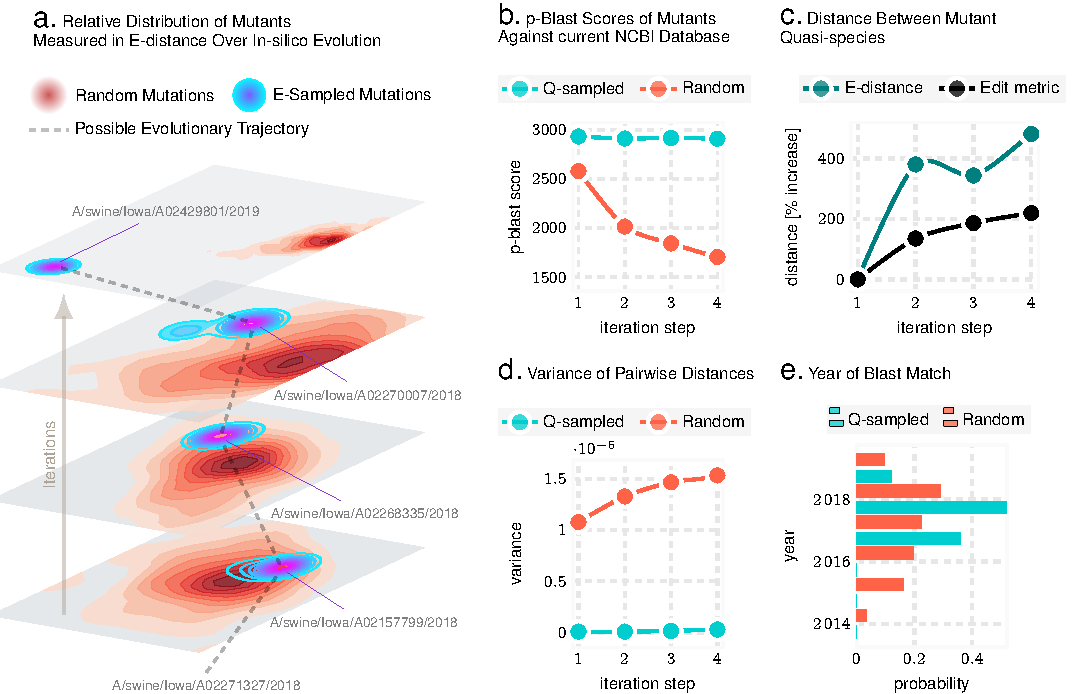
\includegraphics[width=0.9\textwidth]{Figures/External/blastvalid.pdf}
  \fi

  \captionN{\textbf{\qdist validation in-silico using Influenza A sequences from NCBI database. Panel a} illustrates that the \enet induced modeling of evolutionary trajectories initiated from known haemagglutinnin (HA)  sequences  are distinct from random paths in the strain space. In particular, random trajectories have more variance, and more importantly, diverge to different regions of the landscape compared to \enet predictions. \textbf{Panels b-e} show that unconstrained Q-sampling  produces sequences maintain a higher degree of similarity to known sequences, as verified by blasting against known HA sequences, have a smaller rate of growth of variance, and produce matches in closer time frames to the initial sequence. \textbf{Panel c} shows that this is not due to simply restricting the  mutational variations, which increases rapidly in both the \enet and the classical metric.}\label{figsoa}
\end{figure*}
\else
\refstepcounter{figure}\label{figsoa}
\fi
%#############################################
%#############################################


%#############################################
%#############################################
%#############################################
\ifFIGS
\begin{figure*}[!ht]
  \centering
  \tikzexternalenable
  \tikzsetnextfilename{dom}

  \iftikzX
  
\begin{tikzpicture}[font=\bf\sffamily\fontsize{8}{8}\selectfont]
\def\DATAA{Figures/plotdata/h1n1humanHA_dom_ldist.dat}
\def\DATAB{Figures/plotdata/h1n1humanNA_dom_ldist.dat}
\def\DATAC{Figures/plotdata/h3n2humanHA_dom_ldist.dat}
\def\DATAD{Figures/plotdata/h3n2humanNA_dom_ldist.dat}

\node[] (A) at (0,0) {
\begin{tikzpicture}
\begin{groupplot}[group style={
        group size=2 by 2,
        xlabels at=edge bottom,
        xticklabels at=edge bottom,
        vertical sep=0.2in, horizontal sep=.35in,
    },height=2in,width=2in]

\nextgroupplot[ylabel=probability,ylabel style={xshift=-.8in,yshift=-.1in}]
\addplot [
    hist={
        bins=50,
        data min=0,
        data max=30,
density=true
    }  , fill=black!50
] table [y index=0] {\DATAA};
\addlegendentry{HA H1N1}


\nextgroupplot[]
\addplot [
    hist={
        bins=50,
        data min=0,
        data max=30,
density=true
    }    , fill=black!50
] table [y index=0] {\DATAB};
\addlegendentry{NA H1N1}


\nextgroupplot[xlabel=Edit Distance from Dominant Strain,xlabel style={xshift=.8in}]
\addplot [
    hist={
        bins=50,
        data min=0,
        data max=30,
density=true
    }    , fill=black!50
] table [y index=0] {\DATAC};
\addlegendentry{HA H3N2}


\nextgroupplot[]
\addplot [
    hist={
        bins=50,
        data min=0,
        data max=30,
density=true
    }    , fill=black!50
] table [y index=0] {\DATAD};
\addlegendentry{NA H3N2}


\end{groupplot}
\end{tikzpicture}
};

\node [anchor=south west] (L1) at (A.north west) {{\large a.} Distribution around dominant strain};

\end{tikzpicture}

  
  \else
  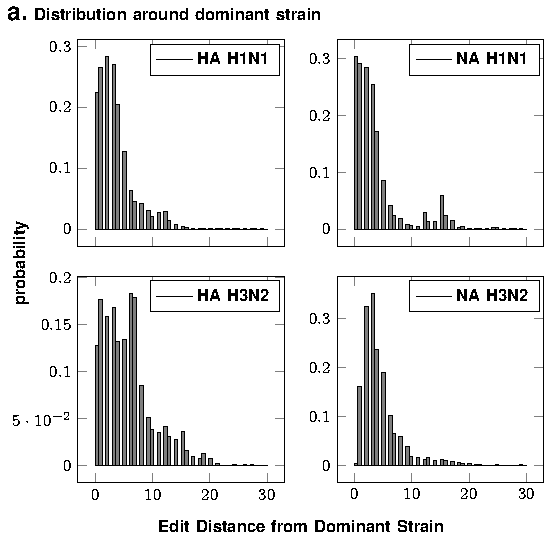
\includegraphics[width=.6\textwidth]{Figures/External/dom.pdf}
  \vspace{0pt}
  \fi
  
\vspace{0pt}

\captionN{\textbf{No. of mutations from the seasonal dominant strain over the years} The quasispecies that circulates each season for each sub-type is tightly distributed around the dominant strain on average.}\label{figdom}
\end{figure*}
\else
\refstepcounter{figure}\label{figdom}
\fi
%#############################################
%#############################################


\clearpage



 \begin{table}\centering
\captionN{H1N1 NA Northern Hemisphere}\label{tabrec4}

\sffamily\fontsize{7}{8}\selectfont

\begin{tabular}{L{.37in}|L{1.62in}|L{1.62in}|L{1.62in}|L{.25in}|L{.25in}}\hline
Year & WHO Recommendation & Dominant Strain & \qnet Recommendation & WHO Error & \qnet Error \\\hline
2001-02& A/New  Caledonia/20/99 & A/New  York/447/2001 & A/Memphis/15/2000 &4&4\\\hline
2002-03& A/New  Caledonia/20/99 & A/Paris/0833/2002 & A/New  York/341/2001 &1&5\\\hline
2003-04& A/New  Caledonia/20/99 & A/Memphis/5/2003 & A/New  York/291/2002 &3&5\\\hline
2004-05& A/New  Caledonia/20/99 & A/Singapore/14/2004 & A/New  York/223/2003 &2&3\\\hline
2005-06& A/New  Caledonia/20/99 & A/Taiwan/5524/2005 & A/Florida/3e/2004 &3&0\\\hline
2006-07& A/New  Caledonia/20/99 & A/Massachusetts/08/2006 & A/Sofia/361/2005 &4&2\\\hline
2007-08& A/Solomon  Islands/3/2006 & A/Tennessee/UR06-0106/2007 & A/Sofia/490/2006 &9&2\\\hline
2008-09& A/Brisbane/59/2007 & A/Sendai/TU66/2008 & A/Maryland/04/2007 &0&3\\\hline
2009-10& A/Brisbane/59/2007 & A/Thailand/SR08021/2009 & A/Paris/910/2008 &87&87\\\hline
2010-11& A/California/7/2009 & A/Finland/2460N/2010 & A/Rome/709/2009 &2&9\\\hline
2011-12& A/California/7/2009 & A/Tula/CRIE-GSYu/2011 & A/Oman/SQUH-40/2010 &4&2\\\hline
2012-13& A/California/7/2009 & A/Bangalore/697-32/2012 & A/Nizhnii  Novgorod/CRIE-ZCA/2011 &4&0\\\hline
2013-14& A/California/7/2009 & A/Jiangsugusu/SWL1824/2013 & A/LongYan/SWL33/2013 &5&3\\\hline
2014-15& A/California/7/2009 & A/LongYan/SWL2457/2014 & A/Utah/06/2013 &9&3\\\hline
2015-16& A/California/7/2009 & A/Michigan/45/2015 & A/Maryland/02/2014 &14&4\\\hline
2016-17& A/California/7/2009 & A/Mexico/4436/2016 & A/India/Pun151245/2015 &14&0\\\hline
2017-18& A/Michigan/45/2015 & A/Illinois/37/2017 & A/Utah/02/2016 &3&3\\\hline
2018-19& A/Michigan/45/2015 & A/Kenya/47/2018 & A/Maine/24/2017 &4&0\\\hline
2019-20& A/Brisbane/02/2018 & A/Texas/7939/2019 & A/Missouri/03/2018 &1&0\\\hline
2020-21& A/Hawaii/70/2019 &A/Togo/897/2020& A/Texas/112/2019 &0&5\\\hline
2021-22& A/Victoria/2570/2019 &A/Cote\_d'Ivoire/3729/2021&A/Togo/0071/2021&1&5\\\hline
2022-23& -1 &-1& A/Lyon/820/2021 &-1&-1\\\hline
\end{tabular}

\flushleft

\fontsize{7}{7}\selectfont
$^\star$ Dominant strain is calculated as the one closest to the centroid in the strain space that year in the edit distance metric
\end{table}


\begin{table}\centering
\captionN{H1N1 NA Southern Hemisphere}\label{tabrec5}

\sffamily\fontsize{7}{8}\selectfont

\begin{tabular}{L{.37in}|L{1.62in}|L{1.62in}|L{1.62in}|L{.25in}|L{.25in}}\hline
Year & WHO Recommendation & Dominant Strain & \qnet Recommendation & WHO Error & \qnet Error \\\hline
2001-02& A/New  Caledonia/20/99 & A/New  York/447/2001 & A/Canterbury/37/2000 &4&6\\\hline
2002-03& A/New  Caledonia/20/99 & A/Paris/0833/2002 & A/New  York/447/2001 &1&5\\\hline
2003-04& A/New  Caledonia/20/99 & A/Memphis/5/2003 & A/New  York/291/2002 &3&5\\\hline
2004-05& A/New  Caledonia/20/99 & A/Singapore/14/2004 & A/Memphis/5/2003 &2&3\\\hline
2005-06& A/New  Caledonia/20/99 & A/Taiwan/5524/2005 & A/Canterbury/106/2004 &3&6\\\hline
2006-07& A/New  Caledonia/20/99 & A/Massachusetts/08/2006 & A/Sofia/361/2005 &4&2\\\hline
2007-08& A/New  Caledonia/20/99 & A/Tennessee/UR06-0106/2007 & A/Thailand/RMSC-UDN-20/2006 &4&8\\\hline
2008-09& A/Solomon  Islands/3/2006 & A/Sendai/TU66/2008 & A/Tennessee/UR06-0151/2007 &15&13\\\hline
2009-10& A/Brisbane/59/2007 & A/Thailand/SR08021/2009 & A/Nebraska/07/2008 &87&87\\\hline
2010-11& A/California/7/2009 & A/Finland/2460N/2010 & A/Rome/709/2009 &2&9\\\hline
2011-12& A/California/7/2009 & A/Tula/CRIE-GSYu/2011 & A/Finland/2460N/2010 &4&2\\\hline
2012-13& A/California/7/2009 & A/Bangalore/697-32/2012 & A/Tula/CRIE-GSYu/2011 &4&0\\\hline
2013-14& A/California/7/2009 & A/Jiangsugusu/SWL1824/2013 & A/Oman/SQUH-63/2012 &5&4\\\hline
2014-15& A/California/7/2009 & A/LongYan/SWL2457/2014 & A/NanPing/SWL1640/2013 &9&6\\\hline
2015-16& A/California/7/2009 & A/Michigan/45/2015 & A/LongYan/SWL2457/2014 &14&5\\\hline
2016-17& A/California/7/2009 & A/Mexico/4436/2016 & A/Michigan/45/2015 &14&0\\\hline
2017-18& A/Michigan/45/2015 & A/Illinois/37/2017 & A/Mexico/4436/2016 &3&3\\\hline
2018-19& A/Michigan/45/2015 & A/Kenya/47/2018 & A/Kentucky/26/2017 &4&2\\\hline
2019-20& A/Michigan/45/2015 & A/Texas/7939/2019 & A/Kenya/47/2018 &4&0\\\hline
2020-21& A/Brisbane/02/2018 &A/Togo/897/2020& A/Texas/7939/2019 &6&5\\\hline
2021-22& A/Victoria/2570/2019 &A/Cote\_D'Ivoire/1496/2021& A/Togo/0155/2021 &1&7\\\hline
2022-23& -1 &-1& A/Dakar/35/2021 &-1&-1\\\hline
\end{tabular}

\flushleft

\fontsize{7}{7}\selectfont
$^\star$ Dominant strain is calculated as the one closest to the centroid in the strain space that year in the edit distance metric
\end{table}
%#############################################
%#############################################


%#############################################

\begin{table}\centering
\captionN{H3N2 NA Northern Hemisphere}\label{tabrec6}

\sffamily\fontsize{7}{8}\selectfont

\begin{tabular}{L{.37in}|L{1.62in}|L{1.62in}|L{1.62in}|L{.25in}|L{.25in}}\hline
Year & WHO Recommendation & Dominant Strain & \qnet Recommendation & WHO Error & \qnet Error \\\hline
2003-04&A/Moscow/10/99& A/Denmark/107/2003 & A/New  York/100/2002 &13&3\\\hline
2004-05& A/Fujian/411/2002 &A/Hyogo/36/2004& A/New  York/20/2003 &3&16\\\hline
2005-06& A/California/7/2004 & A/Denmark/203/2005 & A/Hong  Kong/HKU20/2004 &4&0\\\hline
2006-07& A/Wisconsin/67/2005 & A/Berlin/32/2006 & A/Mexico/InDRE2227/2005 &1&1\\\hline
2007-08& A/Wisconsin/67/2005 & A/Brazil/80/2007 & A/Baden-Wuerttemberg/17/2006 &8&7\\\hline
2008-09& A/Brisbane/10/2007 & A/Missouri/05/2008 & A/Washington/01/2007 &3&2\\\hline
2009-10& A/Brisbane/10/2007 & A/Oklahoma/09/2009 & A/Wisconsin/24/2008 &3&1\\\hline
2010-11& A/Perth/16/2009 & A/California/17/2010 & A/New  York/70/2009 &2&3\\\hline
2011-12& A/Perth/16/2009 & A/Texas/14/2011 & A/California/14/2010 &3&2\\\hline
2012-13& A/Victoria/361/2011 & A/New  York/02/2012 & A/Singapore/C2011.493/2011 &4&1\\\hline
2013-14& A/Victoria/361/2011 & A/Michigan/02/2013 & A/New  York/01/2012 &3&1\\\hline
2014-15& A/Texas/50/2012 & A/Tehran/69634/2014 & A/Boston/DOA2-176/2013 &3&1\\\hline
2015-16& A/Switzerland/9715293/2013 &A/Parma/471/2015& A/Thailand/CU-B10520/2014 &3&0\\\hline
2016-17& A/Hong  Kong/4801/2014 & A/North  Carolina/62/2016 & A/Delaware/02/2015 &7&2\\\hline
2017-18& A/Hong  Kong/4801/2014 & A/Texas/277/2017 & A/New  York/03/2016 &8&0\\\hline
2018-19& A/Singapore/INFIMH-16-0019/2016 & A/Japan/NHRC\_FDX70352/2018 & A/Colorado/11/2017 &4&3\\\hline
2019-20& A/Kansas/14/2017 & A/Washington/9757/2019 &A/Guangxi-Fangcheng/54/2019&3&11\\\hline
2020-21& A/Hong  Kong/2671/2019 & A/Bangladesh/1004005/2020 & A/Maryland/02/2019 &3&13\\\hline
2021-22& A/Cambodia/e0826360/2020 &A/Stockholm/10/2022& A/Bangladesh/1916/2020 &2&2\\\hline
2022-23& -1 &-1& A/Iowa/20/2022 &-1&-1\\\hline
\end{tabular}

\flushleft

\fontsize{7}{7}\selectfont
$^\star$ Dominant strain is calculated as the one closest to the centroid in the strain space that year in the edit distance metric
\end{table}
%#############################################

%#############################################

\begin{table}\centering
\captionN{H3N2 NA Southern Hemisphere}\label{tabrec7}

\sffamily\fontsize{7}{8}\selectfont

\begin{tabular}{L{.37in}|L{1.62in}|L{1.62in}|L{1.62in}|L{.25in}|L{.25in}}\hline
Year & WHO Recommendation & Dominant Strain & \qnet Recommendation & WHO Error & \qnet Error \\\hline
2003-04&A/Moscow/10/99& A/Denmark/107/2003 & A/New  York/101/2002 &13&3\\\hline
2004-05& A/Fujian/411/2002 &A/Hyogo/36/2004& A/New  York/20/2003 &3&16\\\hline
2005-06& A/Wellington/1/2004 & A/Denmark/203/2005 & A/Wellington/1/2004 &2&2\\\hline
2006-07& A/California/7/2004 & A/Berlin/32/2006 & A/Mexico/InDRE2227/2005 &3&1\\\hline
2007-08& A/Wisconsin/67/2005 & A/Brazil/80/2007 & A/Ohio/06/2006 &8&10\\\hline
2008-09& A/Brisbane/10/2007 & A/Missouri/05/2008 & A/Brazil/80/2007 &3&2\\\hline
2009-10& A/Brisbane/10/2007 & A/Oklahoma/09/2009 & A/Wisconsin/24/2008 &3&1\\\hline
2010-11& A/Perth/16/2009 & A/California/17/2010 & A/New  York/70/2009 &2&3\\\hline
2011-12& A/Perth/16/2009 & A/Texas/14/2011 & A/Virginia/05/2010 &3&2\\\hline
2012-13& A/Perth/16/2009 & A/New  York/02/2012 & A/Texas/14/2011 &4&1\\\hline
2013-14& A/Victoria/361/2011 & A/Michigan/02/2013 & A/New  York/02/2012 &3&3\\\hline
2014-15& A/Texas/50/2012 & A/Tehran/69634/2014 & A/Michigan/02/2013 &3&1\\\hline
2015-16& A/Switzerland/9715293/2013 &A/Parma/471/2015& A/Tehran/69634/2014 &3&2\\\hline
2016-17& A/Hong  Kong/4801/2014 & A/North  Carolina/62/2016 &A/Parma/471/2015&7&2\\\hline
2017-18& A/Hong  Kong/4801/2014 & A/Texas/277/2017 & A/Guangdong/264/2016 &8&0\\\hline
2018-19& A/Singapore/INFIMH-16-0019/2016 & A/Japan/NHRC\_FDX70352/2018 & A/Texas/277/2017 &4&3\\\hline
2019-20& A/Switzerland/8060/2017 & A/Washington/9757/2019 & A/Pennsylvania/317/2018 &10&10\\\hline
2020-21& A/South  Australia/34/2019 & A/Bangladesh/1004005/2020 & A/Washington/9757/2019 &1&13\\\hline
2021-22& A/Hong Kong/2671/2019 &A/India/PUN-NIV301718/2021	& A/India/PUN-NIV301132/2021 &6&4\\\hline
2022-23& -1 &-1& A/Michigan/UOM10045036720/2022 &-1&-1\\\hline
\end{tabular}

\flushleft

\fontsize{7}{7}\selectfont
$^\star$ Dominant strain is calculated as the one closest to the centroid in the strain space that year in the edit distance metric
\end{table}
%#############################################







%#############################################
%#############################################

\begin{table}\centering
\captionN{H1N1 NA Northern Hemisphere (Multi-cluster)}\label{tabrec8}

\sffamily\fontsize{7}{8}\selectfont

\begin{tabular}{L{.37in}|L{1.33in}|L{.25in}|L{.25in}|L{.25in}|L{1.65in}|L{1.65in}}\hline
Year & WHO Recommendation & WHO Error & \qnet Error 1 & \qnet Error 2 & \qnet Recommendation 1 & \qnet  Recommendation 2 \\\hline
2001-02& A/New  Caledonia/20/99 &4&1&6& A/New  South  Wales/26/2000 & A/Canterbury/37/2000 \\\hline
2002-03& A/New  Caledonia/20/99 &1&0&5& A/Wellington/1/2001 & A/New  York/447/2001 \\\hline
2003-04& A/New  Caledonia/20/99 &3&2&8& A/Paris/0833/2002 & A/Taiwan/141/2002 \\\hline
2004-05& A/New  Caledonia/20/99 &2&3&4& A/Memphis/5/2003 & A/Hanoi/1004/2003 \\\hline
2005-06& A/New  Caledonia/20/99 &3&0&1& A/Denmark/130/2004 & A/Paris/650/2004 \\\hline
2006-07& A/New  Caledonia/20/99 &4&2&8& A/Sofia/361/2005 & A/Wellington/11/2005 \\\hline
2007-08& A/Solomon  Islands/3/2006 &9&4&8& A/Sofia/246/2006 & A/New  York/8/2006 \\\hline
2008-09& A/Brisbane/59/2007 &0&13&19& A/Tennessee/UR06-0151/2007 & A/Ohio/UR06-0178/2007 \\\hline
2009-10& A/Brisbane/59/2007 &87&88&90& A/Sendai/TU66/2008 & A/Japan/618/2008 \\\hline
2010-11& A/California/7/2009 &2&1&6& A/South  Carolina/WRAIR1645P/2009 & A/Wisconsin/629-D00809/2009 \\\hline
2011-12& A/California/7/2009 &4&1&3& A/England/21680633/2010 & A/Hangzhou/178/2010 \\\hline
2012-13& A/California/7/2009 &4&1&22& A/Joshkar-Ola/CRIE-BLP/2011 & A/Rio  Grande  do  Sul/578/2011 \\\hline
2013-14& A/California/7/2009 &5&4&13& A/Thailand/MR10580/2012 & A/Mexico/INMEGEN-INER  15/2012 \\\hline
2014-15& A/California/7/2009 &9&3&7& A/Minnesota/02/2013 & A/Helsinki/430/2013 \\\hline
2015-16& A/California/7/2009 &14&4&7& A/Helsinki/808M/2014 & A/Virginia/NHRC430739/2014 \\\hline
2016-17& A/California/7/2009 &14&0&3& A/Michigan/45/2015 & A/Colorado/30/2015 \\\hline
2017-18& A/Michigan/45/2015 &3&3&8& A/Mexico/4436/2016 & A/Arizona/03/2016 \\\hline
2018-19& A/Michigan/45/2015 &4&0&4& A/California/NHRC\_QV11073/2017 & A/Minnesota/35/2017 \\\hline
2019-20& A/Brisbane/02/2018 &1&0&2& A/Kenya/47/2018 & A/Colorado/7682/2018 \\\hline
2020-21& A/Hawaii/70/2019 &0&3&8& A/California/NHRC-OID\_BOX-ILI-0012/2019 & A/Indiana/30/2019 \\\hline
2021-22& A/Victoria/2570/2019 &1&5&51& A/Togo/0071/2021 & A/Yunnan-Mengzi/1462/2020 \\\hline
2022-23& -1 &-1&-1&-1& A/Netherlands/10646/2022 & A/Sydney/234/2022 \\\hline
\end{tabular}
\flushleft

\fontsize{7}{7}\selectfont
$^\star$ Dominant strain is calculated as the one closest to the centroid in the strain space that year in the edit distance metric
\end{table}

%#############################################
%#############################################

\begin{table}\centering
\captionN{H1N1 NA Southern Hemisphere (Multi-cluster)}\label{tabrec9}

\sffamily\fontsize{7}{8}\selectfont

\begin{tabular}{L{.37in}|L{1.33in}|L{.25in}|L{.25in}|L{.25in}|L{1.65in}|L{1.65in}}\hline
Year & WHO Recommendation & WHO Error & \qnet Error 1 & \qnet Error 2 & \qnet Recommendation 1 & \qnet  Recommendation 2 \\\hline
2001-02& A/New  Caledonia/20/99 &4&1&6& A/New  South  Wales/26/2000 & A/Canterbury/37/2000 \\\hline
2002-03& A/New  Caledonia/20/99 &1&0&5& A/Wellington/1/2001 & A/New  York/447/2001 \\\hline
2003-04& A/New  Caledonia/20/99 &3&2&8& A/Paris/0833/2002 & A/Taiwan/141/2002 \\\hline
2004-05& A/New  Caledonia/20/99 &2&3&4& A/Memphis/5/2003 & A/Hanoi/1004/2003 \\\hline
2005-06& A/New  Caledonia/20/99 &3&0&1& A/Denmark/130/2004 & A/Paris/650/2004 \\\hline
2006-07& A/New  Caledonia/20/99 &4&2&8& A/Sofia/361/2005 & A/Wellington/11/2005 \\\hline
2007-08& A/New  Caledonia/20/99 &4&4&8& A/Sofia/246/2006 & A/New  York/8/2006 \\\hline
2008-09& A/Solomon  Islands/3/2006 &15&13&19& A/Tennessee/UR06-0151/2007 & A/Ohio/UR06-0178/2007 \\\hline
2009-10& A/Brisbane/59/2007 &87&88&90& A/Sendai/TU66/2008 & A/Japan/618/2008 \\\hline
2010-11& A/California/7/2009 &2&1&6& A/South  Carolina/WRAIR1645P/2009 & A/Wisconsin/629-D00809/2009 \\\hline
2011-12& A/California/7/2009 &4&1&3& A/England/21680633/2010 & A/Hangzhou/178/2010 \\\hline
2012-13& A/California/7/2009 &4&1&22& A/Joshkar-Ola/CRIE-BLP/2011 & A/Rio Grande do Sul/578/2011 \\\hline
2013-14& A/California/7/2009 &5&4&13& A/Thailand/MR10580/2012 & A/Mexico/INMEGEN-INER  15/2012 \\\hline
2014-15& A/California/7/2009 &9&3&7& A/Minnesota/02/2013 & A/Helsinki/430/2013 \\\hline
2015-16& A/California/7/2009 &14&4&7& A/Helsinki/808M/2014 & A/Virginia/NHRC430739/2014 \\\hline
2016-17& A/California/7/2009 &14&0&3& A/Michigan/45/2015 & A/Colorado/30/2015 \\\hline
2017-18& A/Michigan/45/2015 &3&3&8& A/Mexico/4436/2016 & A/Arizona/03/2016 \\\hline
2018-19& A/Michigan/45/2015 &4&0&4& A/California/NHRC\_QV11073/2017 & A/Minnesota/35/2017 \\\hline
2019-20& A/Michigan/45/2015 &4&0&2& A/Kenya/47/2018 & A/Colorado/7682/2018 \\\hline
2020-21& A/Brisbane/02/2018 &5&2&7& A/California/NHRC-OID\_BOX-ILI-0012/2019 & A/Indiana/30/2019 \\\hline
2021-22& A/Victoria/2570/2019 &1&7&58& A/Togo/0155/2021 & A/Shandong/00204/2021 \\\hline
2022-23& -1 &-1&-1&-1& A/Switzerland/86136/2022 & A/Wisconsin/04/2021 \\\hline
\end{tabular}
\flushleft

\fontsize{7}{7}\selectfont
$^\star$ Dominant strain is calculated as the one closest to the centroid in the strain space that year in the edit distance metric
\end{table}

%#############################################
%#############################################

\begin{table}\centering
\captionN{H3N2 NA Northern Hemisphere (Multi-cluster)}\label{tabrec10}

\sffamily\fontsize{7}{8}\selectfont

\begin{tabular}{L{.37in}|L{1.33in}|L{.25in}|L{.25in}|L{.25in}|L{1.65in}|L{1.65in}}\hline
Year & WHO Recommendation & WHO Error & \qnet Error 1 & \qnet Error 2 & \qnet Recommendation 1 & \qnet  Recommendation 2 \\\hline
2003-04&A/Moscow/10/99&13&4&5& A/Auckland/612/2002 & A/New  York/87/2002 \\\hline
2004-05& A/Fujian/411/2002 &3&16&18& A/New  York/20/2003 & A/New  York/12/2003 \\\hline
2005-06& A/California/7/2004 &4&1&7& A/New  York/358/2004 & A/Singapore/36/2004 \\\hline
2006-07& A/Wisconsin/67/2005 &1&3&8&A/Macau/557/2005& A/Hong  Kong/HKU53/2005 \\\hline
2007-08& A/Wisconsin/67/2005 &8&0&10& A/Wisconsin/42/2006 & A/Wisconsin/44/2006 \\\hline
2008-09& A/Brisbane/10/2007 &3&4&10& A/Missouri/06/2007 & A/Japan/72/2007 \\\hline
2009-10& A/Brisbane/10/2007 &3&1&7& A/Wisconsin/24/2008 & A/Mississippi/UR07-0042/2008 \\\hline
2010-11& A/Perth/16/2009 &2&3&8& A/New  York/70/2009 & A/Japan/883/2009 \\\hline
2011-12& A/Perth/16/2009 &3&2&2& A/California/19/2010 & A/Virginia/05/2010 \\\hline
2012-13& A/Victoria/361/2011 &4&1&12& A/Texas/14/2011 & A/Singapore/GP1684/2011 \\\hline
2013-14& A/Victoria/361/2011 &3&1&5& A/Idaho/38/2012 & A/Pavia/135/2012 \\\hline
2014-15& A/Texas/50/2012 &3&1&1& A/Nevada/05/2013 & A/Michigan/02/2013 \\\hline
2015-16& A/Switzerland/9715293/2013 &3&0&4& A/Nicaragua/6866\_14/2014 & A/Iran/91244/2014 \\\hline
2016-17& A/Hong  Kong/4801/2014 &7&1&25& A/New  Jersey/13/2015 & A/California/NHRC\_BRD41056N/2015 \\\hline
2017-18& A/Hong  Kong/4801/2014 &9&1&4& A/Guangdong/264/2016 & A/Victoria/668/2016 \\\hline
2018-19& A/Singapore/INFIMH-16-0019/2016 &3&2&4& A/Netherlands/3530/2017 & A/Washington/17/2017 \\\hline
2019-20& A/Kansas/14/2017 &3&4&10& A/England/538/2018 & A/California/BRD12490N/2018 \\\hline
2020-21& A/Hong Kong/2671/2019 &3&1&13& A/England/9738/2019 & A/Washington/9757/2019 \\\hline
2021-22& A/Cambodia/e0826360/2020 &2&3&7& A/Laos/527/2021 & A/Michigan/UOM10045655748/2020 \\\hline
2022-23& -1 &-1&-1&-1& A/Maine/02/2022 & A/Michigan/UOM10042819294/2021 \\\hline
\end{tabular}
\flushleft

\fontsize{7}{7}\selectfont
$^\star$ Dominant strain is calculated as the one closest to the centroid in the strain space that year in the edit distance metric
\end{table}

%#############################################
%#############################################

\begin{table}\centering
\captionN{H3N2 NA Southern Hemisphere (Multi-cluster)}\label{tabrec11}

\sffamily\fontsize{7}{8}\selectfont

\begin{tabular}{L{.37in}|L{1.33in}|L{.25in}|L{.25in}|L{.25in}|L{1.65in}|L{1.65in}}\hline
Year & WHO Recommendation & WHO Error & \qnet Error 1 & \qnet Error 2 & \qnet Recommendation 1 & \qnet  Recommendation 2 \\\hline
2003-04&A/Moscow/10/99&13&4&5& A/Auckland/612/2002 & A/New  York/87/2002 \\\hline
2004-05& A/Fujian/411/2002 &3&16&18& A/New  York/20/2003 & A/New  York/12/2003 \\\hline
2005-06& A/Wellington/1/2004 &2&1&7& A/New  York/358/2004 & A/Singapore/36/2004 \\\hline
2006-07& A/California/7/2004 &3&3&8&A/Macau/557/2005& A/Hong  Kong/HKU53/2005 \\\hline
2007-08& A/Wisconsin/67/2005 &8&0&10& A/Wisconsin/42/2006 & A/Wisconsin/44/2006 \\\hline
2008-09& A/Brisbane/10/2007 &3&4&10& A/Missouri/06/2007 & A/Japan/72/2007 \\\hline
2009-10& A/Brisbane/10/2007 &3&1&7& A/Wisconsin/24/2008 & A/Mississippi/UR07-0042/2008 \\\hline
2010-11& A/Perth/16/2009 &2&3&8& A/New  York/70/2009 & A/Japan/883/2009 \\\hline
2011-12& A/Perth/16/2009 &3&2&2& A/California/19/2010 & A/Virginia/05/2010 \\\hline
2012-13& A/Perth/16/2009 &4&1&12& A/Texas/14/2011 & A/Singapore/GP1684/2011 \\\hline
2013-14& A/Victoria/361/2011 &3&1&5& A/Idaho/38/2012 & A/Pavia/135/2012 \\\hline
2014-15& A/Texas/50/2012 &3&1&1& A/Nevada/05/2013 & A/Michigan/02/2013 \\\hline
2015-16& A/Switzerland/9715293/2013 &3&0&4& A/Nicaragua/6866\_14/2014 & A/Iran/91244/2014 \\\hline
2016-17& A/Hong Kong/4801/2014 &7&1&25& A/New  Jersey/13/2015 & A/California/NHRC\_BRD41056N/2015 \\\hline
2017-18& A/Hong Kong/4801/2014 &9&1&4& A/Guangdong/264/2016 & A/Victoria/668/2016 \\\hline
2018-19& A/Singapore/INFIMH-16-0019/2016 &3&2&4& A/Netherlands/3530/2017 & A/Washington/17/2017 \\\hline
2019-20& A/Switzerland/8060/2017 &10&4&10& A/England/538/2018 & A/California/BRD12490N/2018 \\\hline
2020-21& A/South  Australia/34/2019 &1&1&13& A/England/9738/2019 & A/Washington/9757/2019 \\\hline
2021-22& A/Hong Kong/2671/2019 &6&1&49& A/Darwin/11/2021 & A/Hawaii/28/2020 \\\hline
2022-23& -1 &-1&-1&-1& A/Congo/313/2021	 & A/Texas/12723/2022 \\\hline
\end{tabular}
\flushleft

\fontsize{7}{7}\selectfont
$^\star$ Dominant strain is calculated as the one closest to the centroid in the strain space that year in the edit distance metric
\end{table}
%#############################################
% %#############################################

%#############################################
\ifFIGS
%#############################################

\begin{table}[!ht]\centering
\captionN{Influenza A Strains Evaluated by IRAT and Corresponding \enet Computed Current Risk Scores}\label{irattab_current}

\sffamily\fontsize{7}{8}\selectfont

\begin{tabular}{L{1.25in}|L{.35in}|L{.3in}|L{.3in}|L{.3in}|L{.35in}|L{.35in}|L{.35in}|L{.35in}|L{.32in}|L{.3in}|L{.3in}}\hline
Influenza Virus & Subype & IRAT Date &IRAT Emergence Score &IRAT Impact Score &HA Sample &NA Sample &HA \erisk & NA \erisk &Geom. Mean&\qnet Emergence Score&\qnet Impact Score \\\hline
 A/swine/Shandong/1207/2016 &H1N1& Jul  2020 &7.5&6.9&1000&1000&-0.0599&-0.0417&0.0500&5.8&5.8\\\hline
 A/Ohio/13/2017 &H3N2& Jul  2019 &6.6&5.8&1000&1000&-0.0091&-0.0692&0.0251&6.2&6.0\\\hline
 A/Hong  Kong/125/2017 &H7N9& May  2017 &6.5&7.5&1000&1000&-0.0092&-0.0046&0.0065&6.7&6.6\\\hline
 A/Shanghai/02/2013 &H7N9& Apr  2016 &6.4&7.2&1000&1000&-0.0031&-0.0044&0.0037&6.8&6.6\\\hline
 A/Anhui-Lujiang/39/2018 &H9N2& Jul  2019 &6.2&5.9&58&58&-0.0157&-0.0467&0.0271&6.2&6.0\\\hline
 A/Indiana/08/2011 &H3N2& Dec  2012 &6.0&4.5&1000&1000&-0.0176&-0.0184&0.0180&6.4&6.3\\\hline
 A/California/62/2018 &H1N2& Jul  2019 &5.8&5.7&37&37&-0.2038&-0.0477&0.0986&5.3&5.9\\\hline
 A/Bangladesh/0994/2011 &H9N2& Feb  2014 &5.6&5.4&58&58&-0.0473&-0.4654&0.1484&3.8&3.6\\\hline
 A/Sichuan/06681/2021 &H5N6& Oct  2021 &5.3&6.3&46&46&-0.3443&-0.0600&0.1437&5.1&6.2\\\hline
 A/Vietnam/1203/2004 &H5N1& Nov  2011 &5.2&6.6&48&45&-0.1323&-0.0411&0.0738&5.6&5.8\\\hline
 A/Yunnan/14564/2015 &H5N6& Apr  2016 &5.0&6.6&46&46&-0.2187&-0.0415&0.0953&5.4&6.0\\\hline
 A/Astrakhan/3212/2020 &H5N8& Mar  2021 &4.6&5.2&95&92&-0.2366&-0.5451&0.3591&4.8&6.1\\\hline
 A/Netherlands/219/2003 &H7N7& Jun  2012 &4.6&5.8&1000&1000&-0.1658&-0.4596&0.2760&3.9&4.5\\\hline
 A/American  wigeon/South  Carolina/AH0195145/2021 &H5N1& Mar  2022 &4.4&5.1&48&45&-0.2355&-0.3135&0.2717&4.3&5.2\\\hline
 A/Jiangxi-Donghu/346/2013$^{\star\star}$ &H10N8& Feb  2014 &4.3&6.0&&&-0.2097&-0.2299&0.2196&4.2&4.8\\\hline
 A/gyrfalcon/Washington/ 41088/2014 &H5N8& Mar  2015 &4.2&4.6&95&92&-0.2387&-0.5438&0.3603&4.8&6.1\\\hline
 A/Northern  pintail /Washington/40964/2014 &H5N2& Mar  2015 &3.8&4.1&95&92&-0.2327&-0.5099&0.3445&4.6&5.8\\\hline
 A/canine/Illinois/12191/2015 &H3N2& Jun  2016 &3.7&3.7&1000&1000&-0.0179&-0.0374&0.0259&6.2&6.1\\\hline
 A/American  green-winged  teal /Washington/1957050/2014 &H5N1& Mar  2015 &3.6&4.1&48&45&-0.2352&-0.3067&0.2686&4.3&5.1\\\hline
 A/turkey/Indiana/1573-2/2016 &H7N8& Jul  2017 &3.4&3.9&1000&1000&-0.0438&-0.4165&0.1351&4.0&3.8\\\hline
 A/chicken/Tennessee/17-007431-3/2017 &H7N9& Oct  2017 &3.1&3.5&1000&1000&-0.0335&-0.5127&0.1310&3.8&3.6\\\hline
 A/chicken/Tennessee/17-007147-2/2017 &H7N9& Oct  2017 &2.8&3.5&1000&1000&-0.0839&-0.5127&0.2075&3.5&3.6\\\hline
 %A/duck/New  York/1996$^\star$ &H1N1& Nov  2011 &2.3&2.4&1000&1000&-1&-1&-1&-1&-1\\\hline
\end{tabular}
\flushleft

\fontsize{8}{8}\selectfont
$^\star$This table contains \enet scores for IRAT computed using current sequence data, thereby computing the current risk of these strains.  
\end{table}
\else
\refstepcounter{table}\label{irattab_current}
\fi
% #############################################
% #############################################

%#############################################
%#############################################
%#############################################
\begin{table}\centering
\captionN{General linear model evaluating \enet emergence risk predictions against IRAT estimates}\label{tabregGLMemergence}\centering

\mnp{6.5in}{
  \fontsize{8}{8}\selectfont
\verbatiminput{Figures/tabdata/model_emergence_simple.txt}
}
\vskip 2em


\mnp{6.5in}{
  \fontsize{8}{8}\selectfont
\verbatiminput{Figures/tabdata/model_emergence_complex.txt}
}
\end{table}
%#############################################
%#############################################
\begin{table}\centering
\captionN{General linear model evaluating \enet impact risk predictions against IRAT estimates}\label{tabregGLMimpact}\centering

\mnp{6.5in}{
  \fontsize{8}{8}\selectfont
\verbatiminput{Figures/tabdata/model_impact_simple.txt}
}
\vskip 2em


\mnp{6.5in}{
  \fontsize{8}{8}\selectfont
\verbatiminput{Figures/tabdata/model_impact_complex.txt}
}
\end{table}
%#############################################
%#############################################

%#############################################
%#############################################
\begin{table}\centering
\captionN{General linear model for evaluating effect of data diversity on \enet performance}\label{tabreg}\centering

\begin{tabular}{L{1.5in}|L{2in}}\hline
  Variable Name & Description \\\hline
  enet\_complexity & Cumulative number of nodes in all predictors in the corresponding \enet \\\hline
  data\_diversity &  Number of clusters in set of input sequence where each sequence in a specific cluster is separated by at least $5$ mutations from sequences not in the cluster\\\hline
  ldistance\_WHO & Deviation of WHO predicted strain from the dominant strain\\\hline
\end{tabular}
\vskip 2em 

\mnp{6.5in}{
  \fontsize{8}{8}\selectfont
\verbatiminput{Figures/tabdata/model1.txt}
}
\vskip 2em


\mnp{6.5in}{
  \fontsize{8}{8}\selectfont
\verbatiminput{Figures/tabdata/model2.txt}
}
\end{table}
%#############################################